\documentclass[runningheads,a4paper]{llncs}

\usepackage{amssymb}
\setcounter{tocdepth}{3}
\usepackage{graphicx}
\usepackage{url}
\urldef{\mailsa}\path|{pjan520, cchatfield, sharris, rhua440, yhunter, samli, rogerl, rdro117,tehbelinda, bradh, bernhardh, morri, claude}@cse.unsw.edu.au|
\newcommand{\keywords}[1]{\par\addvspace\baselineskip
\noindent\keywordname\enspace\ignorespaces#1}

\begin{document}

\mainmatter 

\title{RoboCup SPL 2014 Champion Team Paper}
\titlerunning{SPL 2014 Champion Team Paper}

\author{
Jayen Ashar
\and Jaiden Ashmore
\and Brad Hall
\and Sean Harris
\and Bernhard Hengst
\and Roger Liu
\and Zijie Mei (Jacky)
\and Maurice Pagnucco
\and Ritwik Roy
\and Claude Sammut
\and Oleg Sushkov
\and Belinda Teh
\and Luke  Tsekouras
}
\authorrunning{Ashar, et. al.}

\institute{
School of Computer Science and Engineering\\
University of New South Wales\\
Sydney 2052 Australia\\
\url{http://www.cse.unsw.edu.au}}

\maketitle

\begin{abstract}
Winning the Robocup SPL World Championship is not accomplished in just one year, nor is it just a matter of writing effective software. Our success can also be attributed to the accumulation of experience since 1999, strong institutional support, and dedicated collaborative teamwork. This paper summarises the key contributing innovations from the time the software was rewritten in 2010, and provides some insight into team organisation. In this paper it is not possible to cover all aspects and intricacies of the complex systems comprising the \emph{rUNSWift} software. We have therefore included an extensive list of references to our technical reports that provide detailed accounts of the research, algorithms and results over the last 5 years.  All the reports are available on one website for easy access and make reference to many external publications, including those from other teams in our league. 
\end{abstract}





\section{Introduction}

Team \emph{rUNSWift} from the University of New South Wales has been competing in the Standard Platform League (SPL) since 1999.  The league was formerly called the Sony Four Legged League. We started as \emph{UNSW United} and were world champions three times in the years 2000 to 2003. It has taken eleven years to regain the world title. In the interim we have seen major changes in both the robots and the field. In 1999 each team played on a 6 $m^2$ field with a border using three first generation ERS-110 Sony AIBO robots. The field was uniformly illuminated to 300 lux and localisation was aided by six beacons and coloured goals. In contrast, the 2014 games were played on a 54 $m^2$ borderless field using standard venue lighting, uniform coloured goals, and without beacons. There are now 6 Aldebaran V4 NAO bipedal robots per side including a coach robot.  

While the SPL prohibits any hardware modification to the robots, fielding a world champion team is not just a matter of good programming. Our experience is that other requirements, including strong institutional support, a cohesive team of motivated participants, a sound strategic plan, regular team meetings, and many hours of testing and debugging are necessary. An additional UNSW challenge is that this is largely a final year project for undergraduates. While we try to encourage participation over several years, the high student turnover means that we have more new recruits faced with a steep learning curve.  

The current rUNSWift software architecture that led to the 2014 win had its genesis in 2010 when the code was rewritten from scratch. Although this report is authored by the 2014 team, their success is a culmination of all the developments from 1999, but particularly since 2010 \cite{tsekouras2014runswift}. The 2014 rUNSWift team members are Luke Tsekouras, Jaiden Ashmore, Zijie Mei (Jacky), Belinda Teh, Oleg Sushkov, Ritwik Roy, Roger Liu, Sean Harris, Jayen Ashar, and faculty members Brad Hall, Bernhard Hengst, Maurice Pagnucco, and Claude Sammut,  several of whom are shown in the photo in Figure \ref{figTeamPhoto2014}.

\begin{figure}
\centering
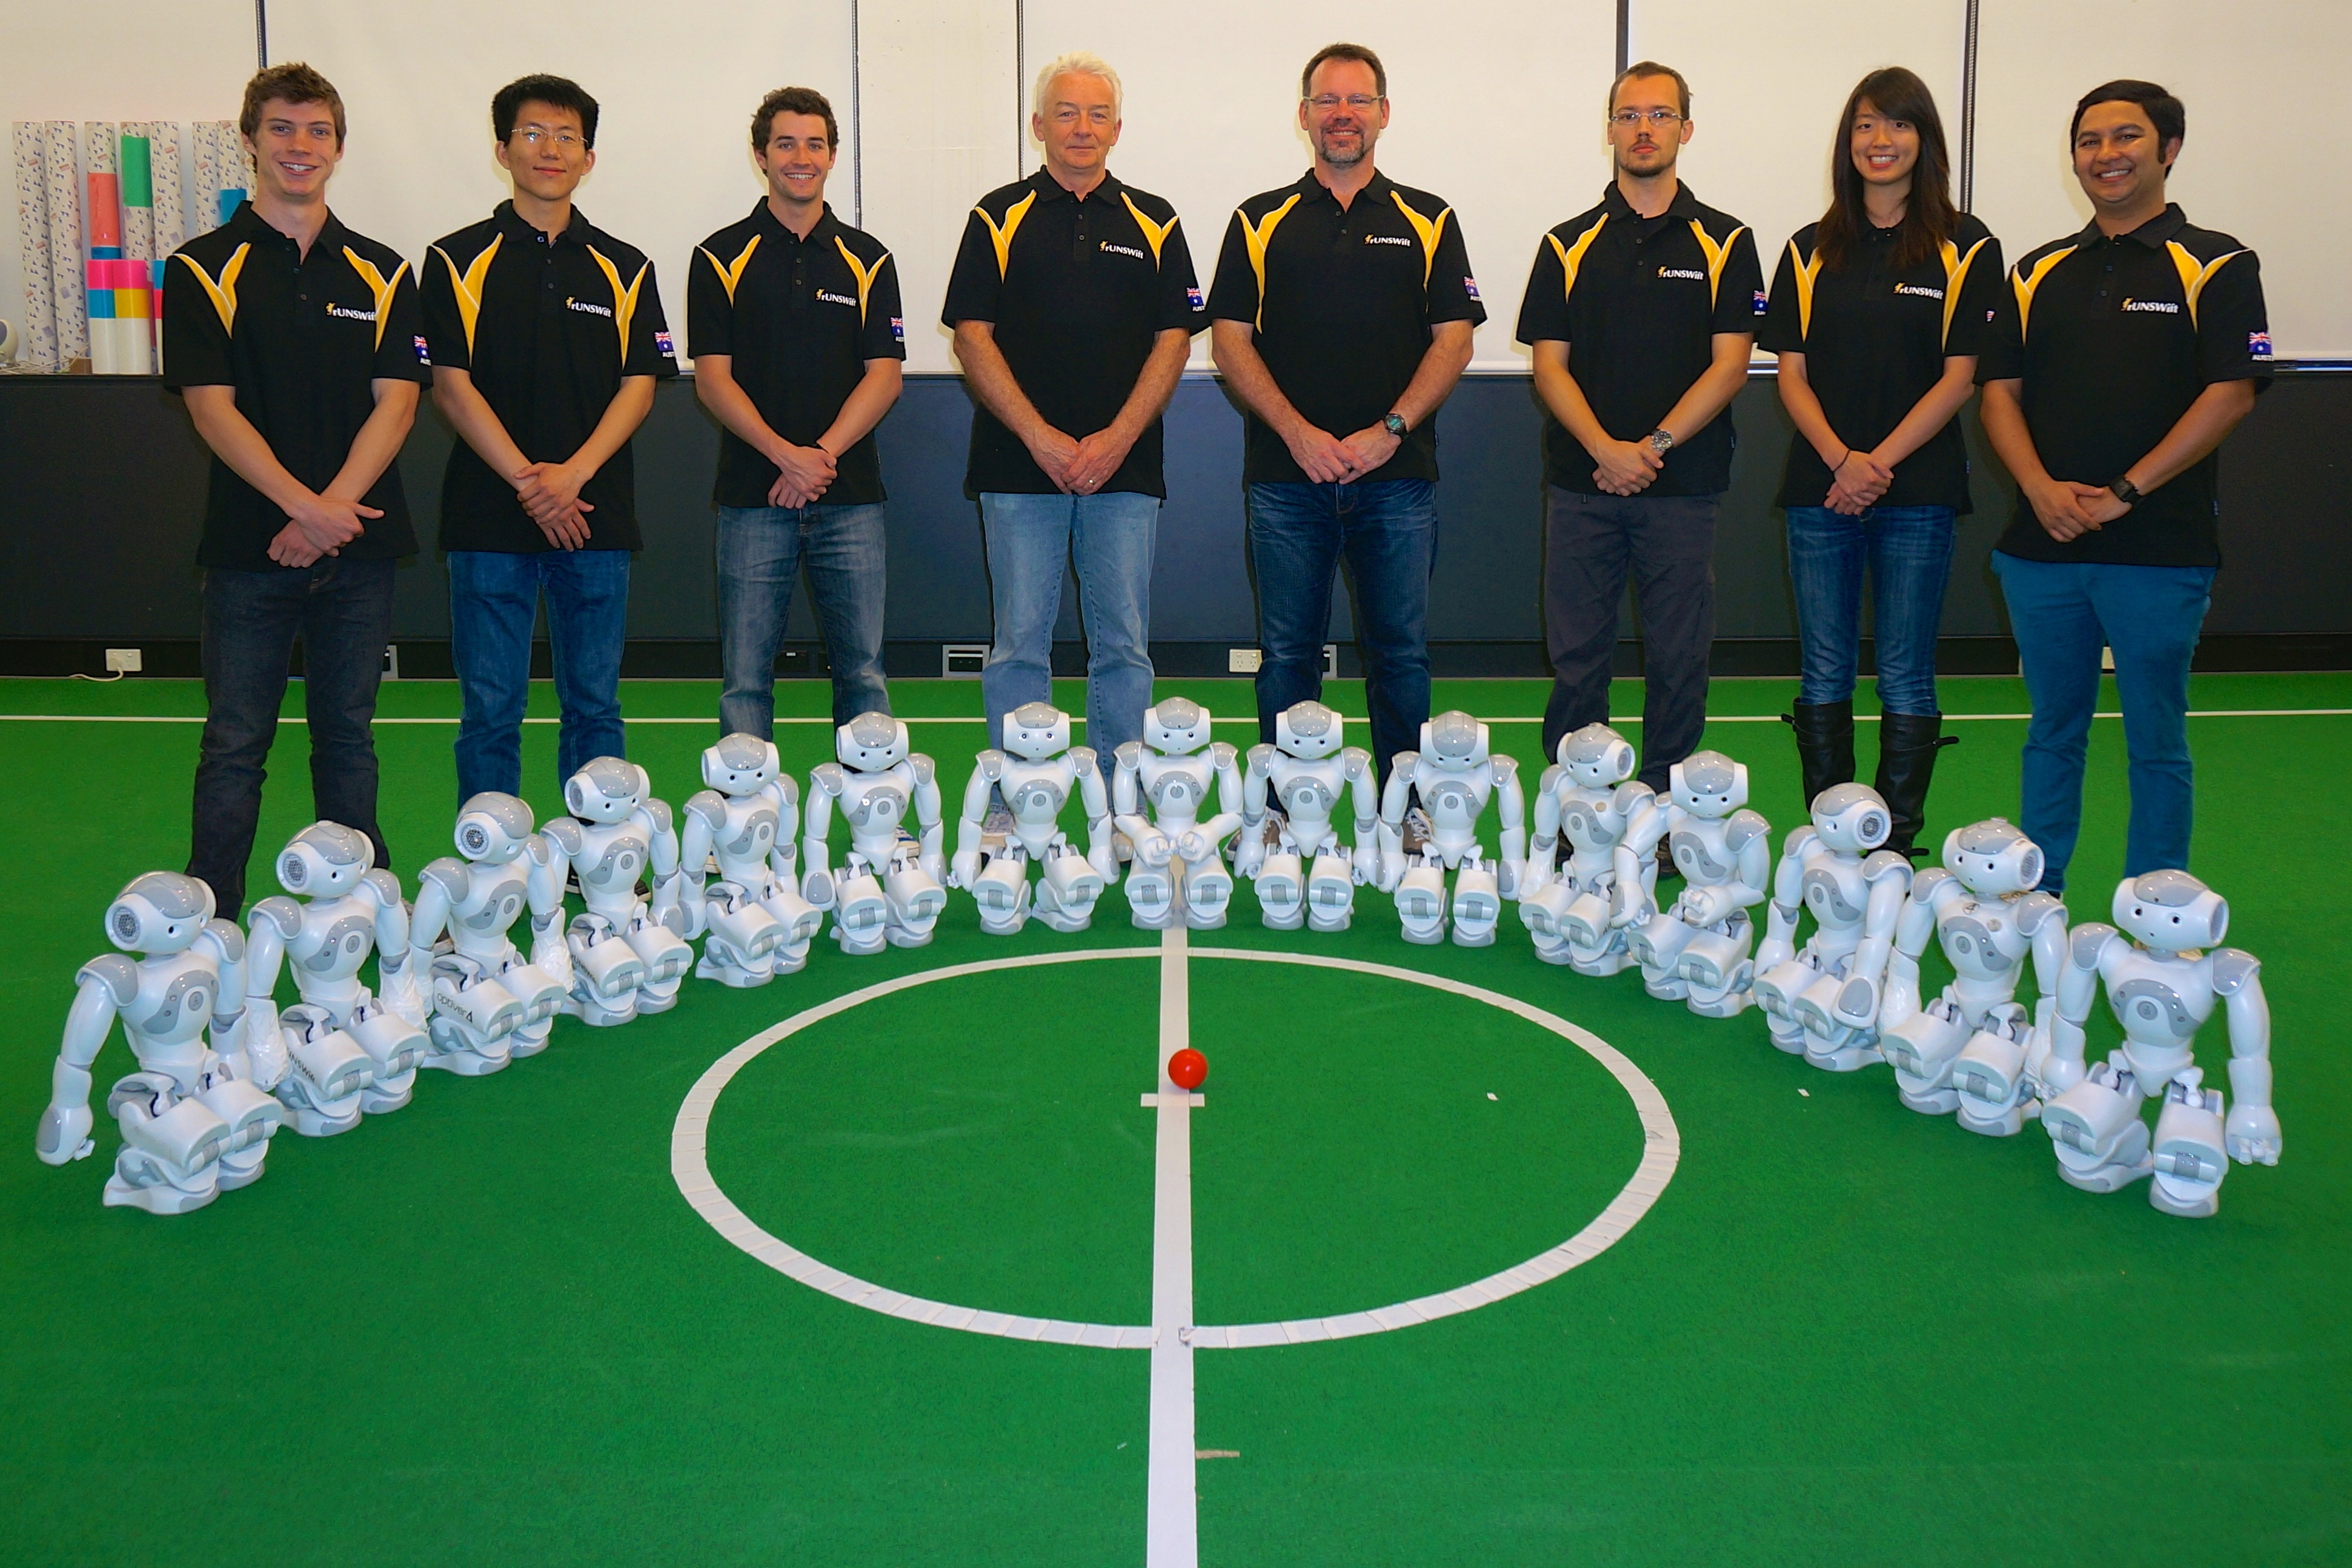
\includegraphics[width=0.8\textwidth]{Figures/figTeamPhoto2014}
\caption{A subset of the 2014 rUNSWift Team. From left to right: Jaiden Ashmore, Zijie Mei (Jacky), Sean Harris, Bernhard Hengst, Brad Hall, Oleg Sushkov, Belinda Teh, Ritwik Roy.} \label{figTeamPhoto2014}
\end{figure}

The objective of this report is therefore to summarise both the technical approach and to describe the team organisation from 2010 to the world championship in 2014. This paper references many UNSW Computer Science and Engineering technical reports that provide detailed information and external references of rUNSWift developments throughout these years. Several of the reports have been published in international publications.\footnote{For completeness all the more than 40 reports are provided in one location at: \\ \url{ http://cgi.cse.unsw.edu.au/~robocup/2014ChampionTeamPaperReports/ }}

The rest of this paper will cover our strategic planning process, the robot and software architectures, the major functional modules of perception, localisation, motion, and behaviour, our team organisation, and future work in the pipeline. 







\section{Strategic Planning and Development Methodology}

Each year the new team plans developments using storyboards or just itemising objectives. For example, the 2010 version 1 storyboard \cite{hengst2010robocupstoryboard} included innovations such as a camera preprocessing stage we call the \emph{saliency image} to reduce the vision processing load, and the RANSAC matching of outer field-edges with straight lines as additional field features. 

Ensuing developments included visual identification of natural landmarks, foveated vision, iterative closest point combination of visual features, decision-tree learning of robot recognition, several iterations of multi-modal Kalman filters for localisation, and new motions for walking and kicking. 

The 2014 strategy called for a major overhaul of the omni-directional locomotion, upgrade of the vision system to use higher definition  camera images for field feature and goal detection, improved robot recognition, the reintroduction of a distributed multi-modal Kalman filter for localisation, and the rewriting of behaviours to improve robot team play on the large field. 

Projects are selected by team participants based on interest and priority. New developments need to demonstrate improvement before being accepted into the code-base. 

The development methodology mantra reinforced each year and adopted by the teams is ``fail-fast, fail cheap".  Our research strategy demands a complete integrated system at each stage, accepting poor performance initially, but quickly iterating through improved versions. 







\section{Robot Architecture}

Figure \ref{figRobotArchitecture} is a schematic of the rUNSWift robotic architecture showing the functional elements of sensor processing, world-modelling, and behaviour generation. This robotic architecture was first employed in 2000 \cite{hengst2000unswunited} and has stood the test of time. 

\begin{figure}[!htp]
\centering
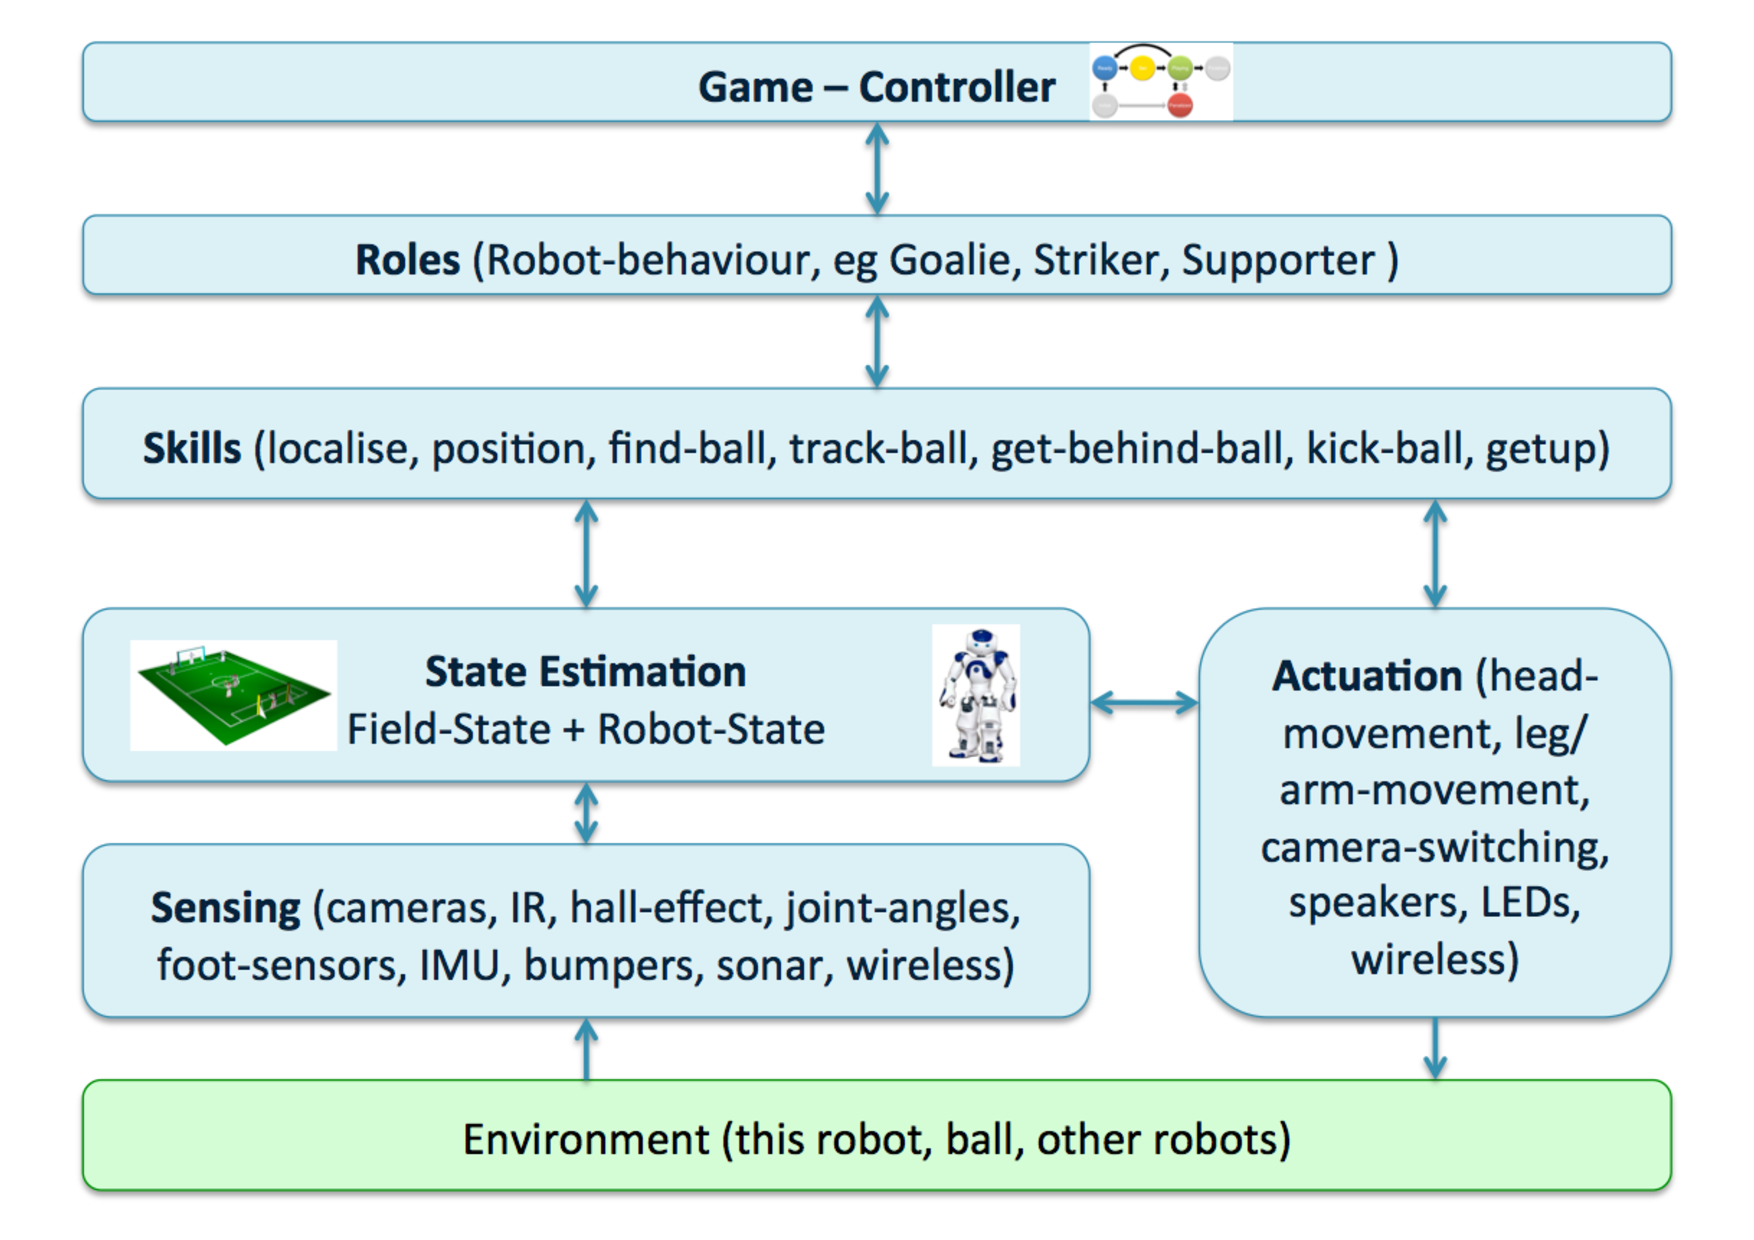
\includegraphics[width=0.8\textwidth]{Figures/figRobotArchitecture}
\caption{The rUNSWift robotic architecture.} \label{figRobotArchitecture}
\end{figure}

The rUNSWift robotic architecture can be envisaged as a \emph{task-hierarchy} that consists of a set of finite state machines linked in a hierarchical lattice. The architecture is distributed in that each NAO robot tracks its own world-model rather than having one commander robot with a centralised view. This provides a level of redundancy in case individual robots are disqualified or stop working. Robots may have slightly different beliefs about the world formed from partially observable and noisy inputs. Robots share their world-model by communicating their position and that of the ball through wireless communication. 

At the root-level, the game-controller changes the states of the game and player robots determine their roles implicitly from their world model. 






\section{Software Architecture}

The Aldebaran NAO robot is equipped with a Linux operating system, as well as custom software from Aldebaran called \emph{NaoQi} which allows interaction with the hardware. The \emph{Device Communications Manager} (DCM) module of NaoQi actuates the joints and LEDs of the robot and reads sensors, including joint angle sensors, accelerometers, and sonars. We deploy two separate binary packages on the robot: \emph{libagent} and \emph{runswift}, which communicate using a block of shared memory and a semaphore. 

The primary purpose of libagent is to provide an abstraction layer over the DCM that has the task of reading sensors and writing actuation requests. To facilitate in-game debugging, without the need to connect an external computer to the robot, a variety of features were added to libagent. These included a system of button-presses to perform various actions, such as releasing stiffness or running system commands. The libagent module also takes over the use of the LEDs for debugging purposes. 

The \emph{runswift} binary is a stand-alone linux executable, detached from NaoQi for safety and debugging. It reads frames from the two cameras, reads and writes to a shared memory block, synchronises with libagent to read sensor values and write actuation commands, and performs all the necessary processing to have the NAO robot play soccer. Because it is detached from NaoQi, it is easy to run runswift off-line, with the Motion thread disabled, allowing for vision processing and other testing to take place without physical access to a robot. It can be run using any of the standard linux debugging wrapper programs. The \emph{runswift} executable is a multi-threaded process. The 6 threads are: Perception, Motion, Off-Nao Transmitter, NAO Transmitter, NAO Receiver and GameController Receiver. 

The Perception thread is responsible for processing images, localising, and deciding actions using the behaviour module. The Motion thread is a near real-time thread, synchronised with libagent, and therefore the DCM, that computes appropriate joint values using the current action command and sensor values. The other threads are all networking related. A blackboard is used to share information internally between threads and externally between robots. We broadcast serialised blackboard information from each robot at 5 Hz to each of its team-mates and Off-Nao.

Off-Nao is a desktop robot monitoring application which streams data from the NAO using a TCP/IP connection. Recordings can be reviewed in Off-Nao, to help determine the relationship between a sequence of observations and the resulting localisation status determined on the robot, as well as other correlations not determinable in real-time.

To facilitate the rapid development of behaviours, we chose to use Python. The Python interpreter was embedded into the \emph{runswift} C++ executable. We monitor a directory on the robot containing Python code, and reload the interpreter whenever the Python code changes. Writing behaviours in a dynamic auto-reloadable language such as Python, means higher  team productivity.

The software architecture developed in 2010 has largely been retained. More detailed information can be found in several reports \cite{cse10rUNSWift2010}  \cite{claridge2011generationpython} and the 2010 code release \cite{claridge2010runswiftcoderelease}.





\section{Perception}

Vision is the primary sensor on the NAO and the one that consumes most of the computational resources. To stay within our processing budget, we sub-sample image pixels in a regular grid pattern to form a \emph{saliency image} that is scanned for features of interest. 

Unable to rely on colour alone due to poorer venue lighting we have added image edges as an additional modality to help identify objects. We still perform manual colour calibration, but supplement the colour-classified image with a gray-scale gradient image. Once points of interest have been identified, higher resolution rectangular foveas are used to focus processing resources while concurrently tracking several field features and ball hypotheses. In this way we can, for example, identify the ball from over half the field length away.  Figure \ref{figBallDetection} shows the accurate detection of a distant poorly colour-classified ball. Related reports include \cite{cse10rUNSWift2010}, \cite{hengst10robocup}, \cite{chatfield2011foveated}, and \cite{ratter2011fast}.

\begin{figure} [h]
\centering
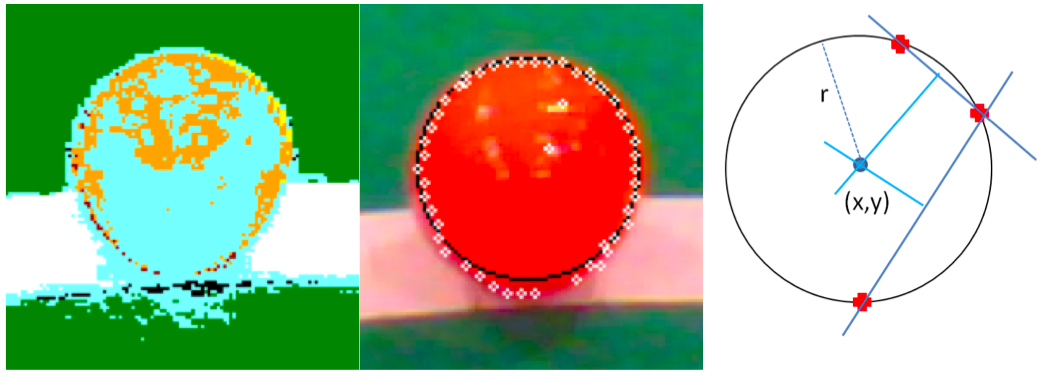
\includegraphics[width=0.8\textwidth]{Figures/figBallDetection}
\caption{Ball detection using colour and gradient in a high-resolution rectangular fovea 
} \label{figBallDetection}
\end{figure}


\begin{figure} [h]
\centering
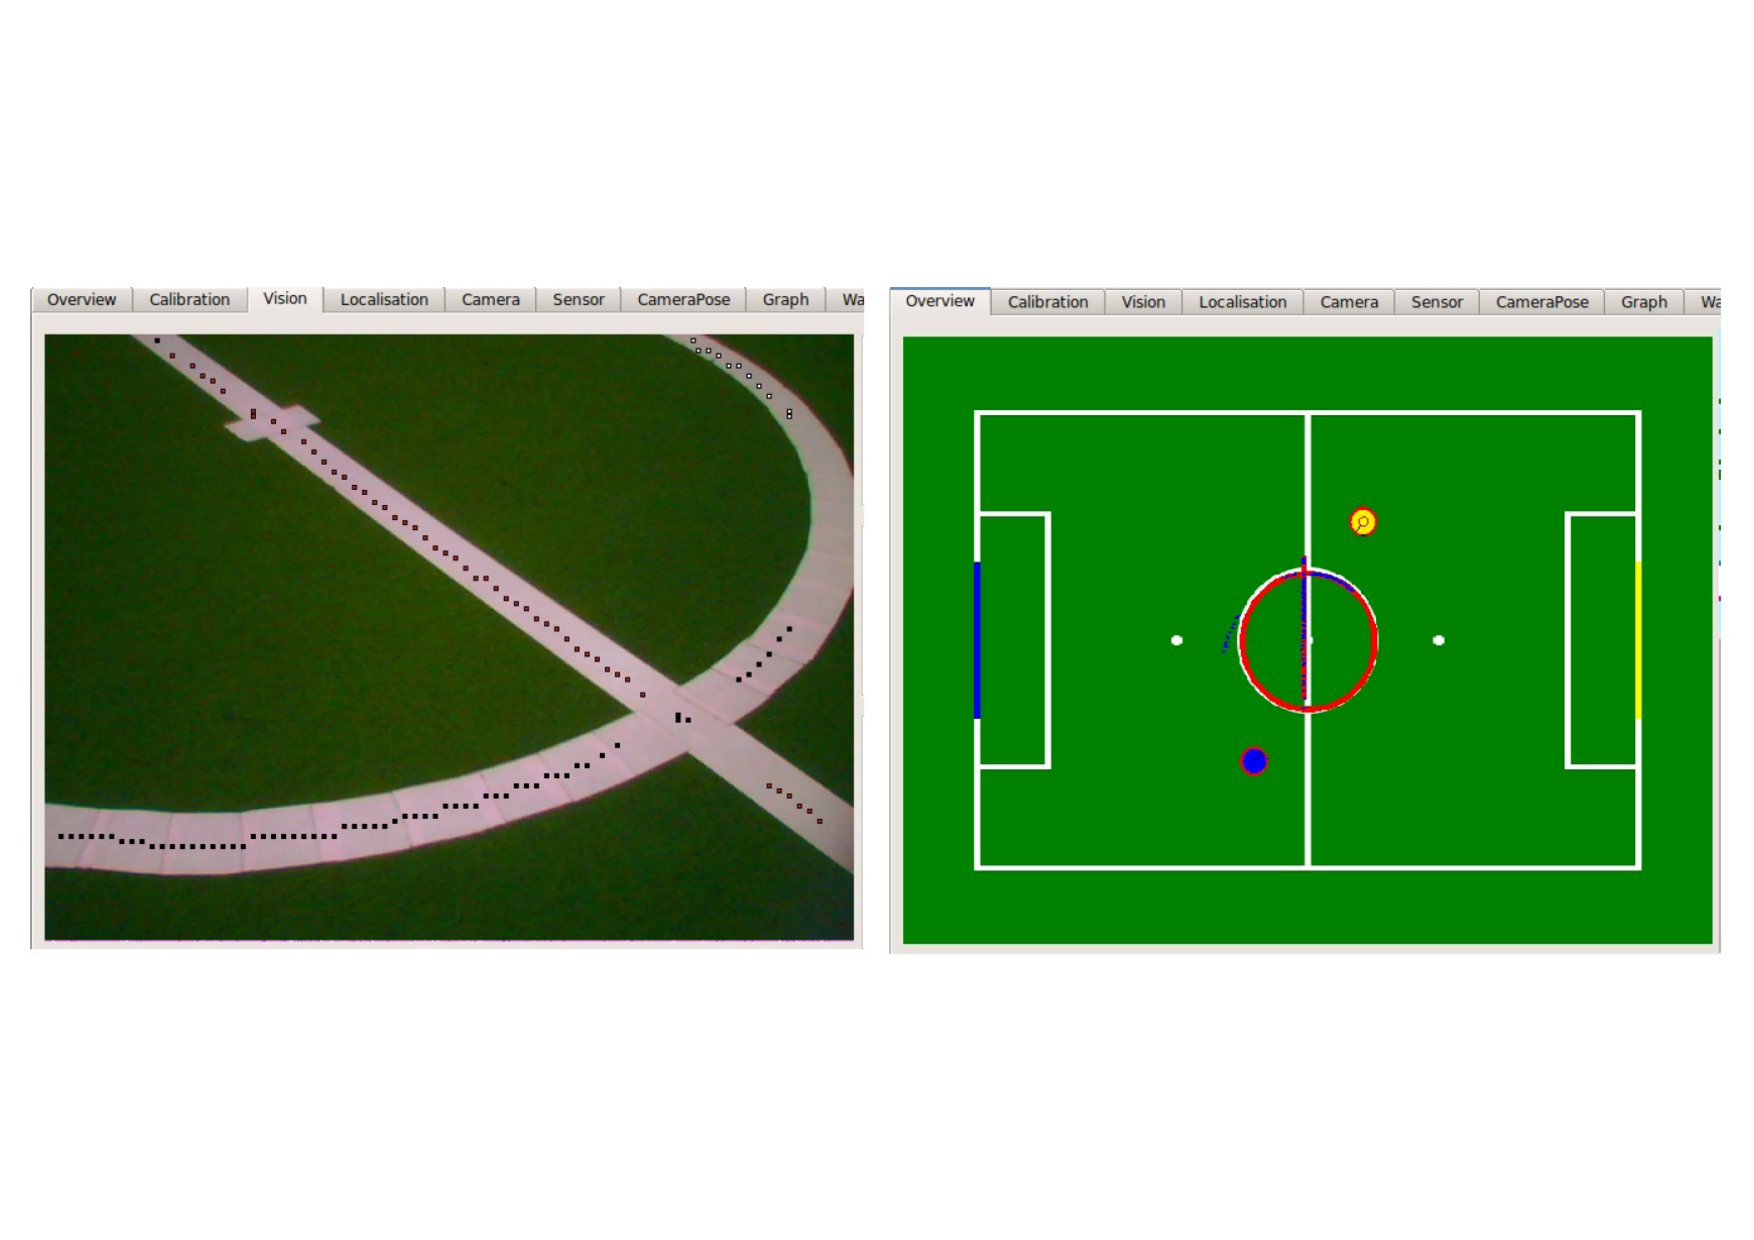
\includegraphics[width=0.8\textwidth]{Figures/figLineCircleRANSAC}
\caption{Detecting field lines and the centre circle simultaneously using RANSAC} 
\label{figLineCircleRANSAC}
\end{figure}

RANSAC field-edge detection in 2010 was extended to field-line detection in 2011 \cite{harris2011featureransac}. The extension uses image colour and gradient to identify both straight lines and the centre circle with a novel RANSAC algorithm that concurrently detects both features reliably (Figure \ref{figLineCircleRANSAC}). Composite feature corners, T-intersections and parallel lines are passed to localisation via a unified sensor observation for the correction cycle of the Kalman filter. 

\begin{figure} [h]
\centering
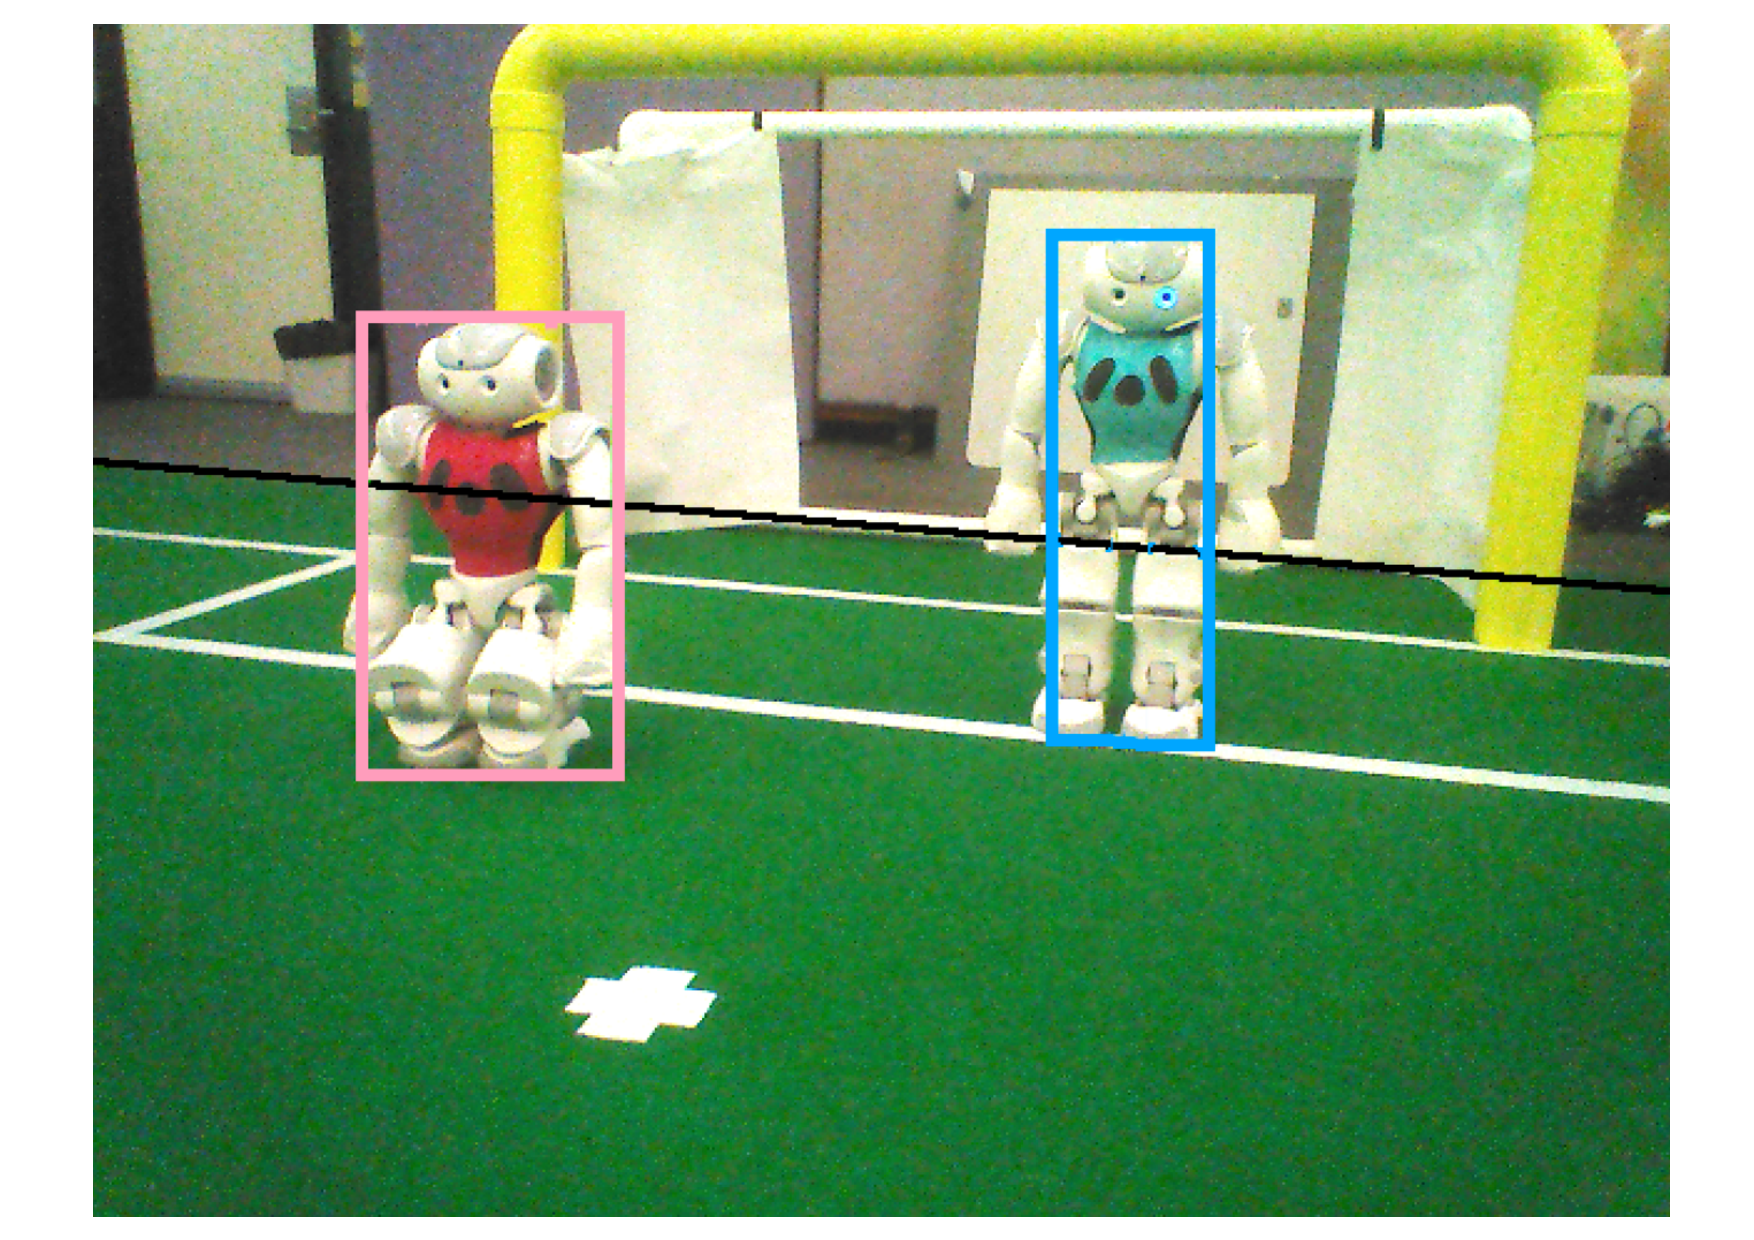
\includegraphics[width=0.6\textwidth]{Figures/figRobotDetection}
\caption{Robot Detection using a Naive Bayes Classifier.} 
\label{figRobotDetection}
\end{figure}

Our vision robot detection algorithm has been subjected to several iterations over the years and together with sonar has been successful in detecting close robots. A region based approach in 2010 \cite{cse10rUNSWift2010} was replaced by machine learning a decision tree from multi-modal vision features in 2011 \cite{kurniawan2011modalrobotdetection} and improved using a naive Bayes classifier in 2014  \cite{ashmore2014robotdetection} (Figure \ref{figRobotDetection}). At close range we experimented with just foot detection using a Hough transform \cite{youssef2011industrial} but this development is not included in the current code.

\begin{figure} [h]
\centering
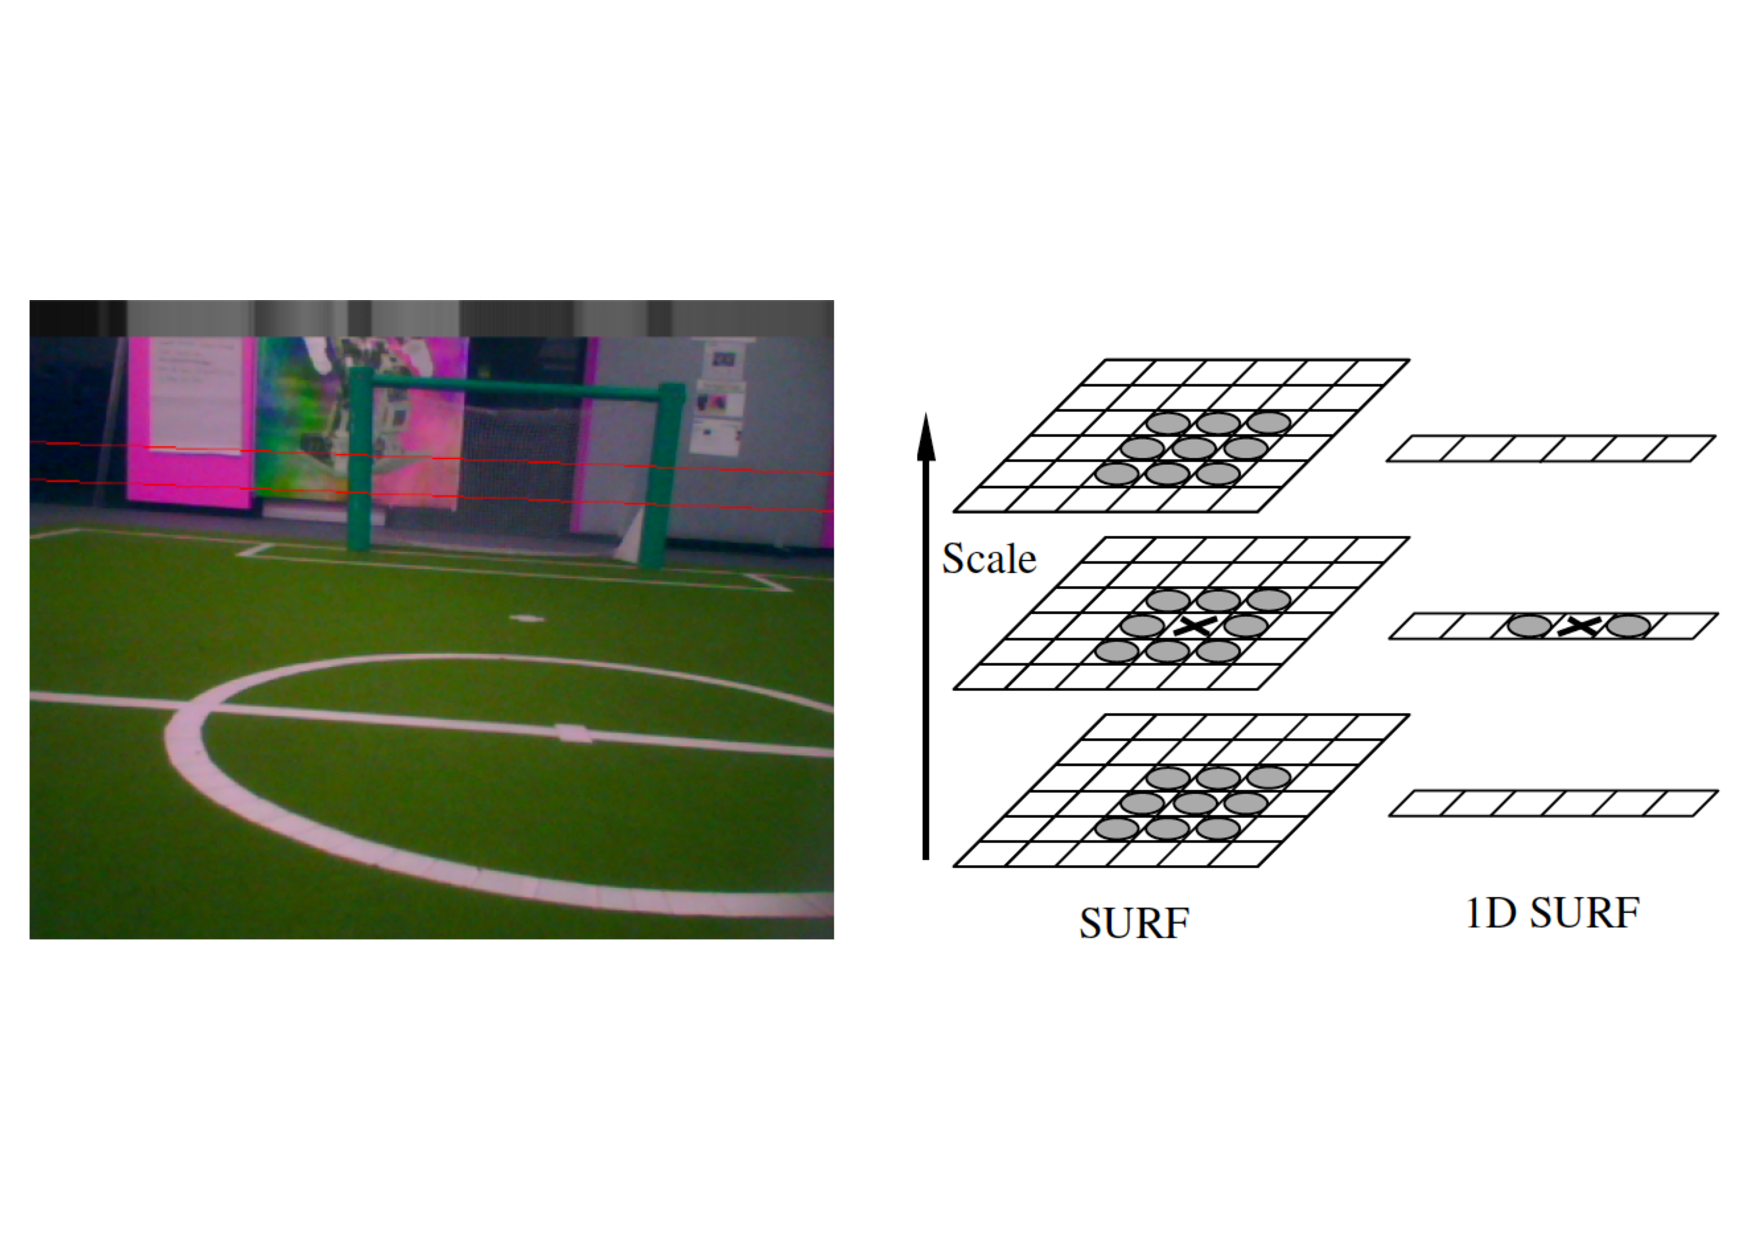
\includegraphics[width=0.8\textwidth]{Figures/figSURF1D}
\caption{Natural Landmarks. A strip of image pixels at robot eye level (between the red lines) is reproduced at the top of the image in gray-scale to find 1D SURF features.} 
\label{figSURF1D}
\end{figure}

The uniform coloured goals require methods for distinguishing the otherwise aliased ends of the field. A 2011 attempt was to use the zero-crossing points of the gradient image at the level of the horizon to map background features \cite{deng2011natural}. In 2012 a one dimensional version of the local feature point detector SURF, was found to be three orders of magnitude faster than the 2D version and viable on the NAO. With a distinguishing visual pattern at robot eye level behind the goals, robots were again able to tell the ends of the field apart (Figure \ref{figSURF1D}) \cite{anderson2012robot}, \cite{anderson2012improvingperception}, \cite{anderson2012naturallandmark}. The technique has been extended to a full 360 degree visual compass \cite{anderson2014fast}. 



A unified field-feature sensor model utilises the extra information available from the specific combination of observed features. 2010 saw early incarnations of sensor models that use multiple goal-posts and field-edges \cite{cse10rUNSWift2010}. In 2012 all the observed features were combined using a modified iterative closest point (ICP) algorithm that resulted in significant improvements in localisation accuracy \cite{harris2012robocup} \cite{anderson2013icpsensormodel}.





\section{Localisation}

We used the combination of a particle filter (to solve the kidnapped robot problem) and a Kalman filter for localisation in 2010. In 2011 a multi-hypothesis linear Kalman filter with a mode selection algorithm using the combined field feature sensor model proved to be accurate and reliable \cite{claridge2011multihypothesiskf}. In that year we also developed a separate Kalman filter model to track a moving ball \cite{teh2011ballmodelling}. 

It is often difficult to measure the ground truth adequately when evaluating localisation algorithms. An exemplary effort in 2011 found a method for tracking a NAO robot in real-time by un-distorting and stitching together two fish-eye images of the field from cameras mounted on our low ceiling in the lab \cite{jisarojito2011trackingoverhead}.

From 2012 onwards goal colours were uniform. A combination of natural feature detection, the unified field-sensor model, using the ball as a disambiguation beacon and a multi-modal Kalman filter ensured accurate localisation \cite{hunter2012localisation}.  No own-goals were scored throughout the entire competition that year.

In 2014 our approach to localisation combined the ICP unified field-sensor model with a distributed multi-modal Kalman filter, which is used for tracking the belief-state of all the robot positions on the field. One of the key features of this localisation system is distributed state tracking. Robots combine their observations via wireless communication to track the full global state of the team, including the ball, with the one filter. This Kalman filter algorithm is based on the successful AIBO 2006 rUNSWift localisation system  \cite{sushkov2006robotlocalisation}.






\section{Motion}
The two new omni-directional walking motions developed in 2010 were \emph{SlowWalk} and \emph{FastWalk} \cite{cse10rUNSWift2010}.  SlowWalk is an open-loop walk that maintains balance by keeping the center-of-mass over the support polygon of the stance foot. This walk formed the basis of several variable strength kicking behaviours. Fastwalk is a closed-loop walk based on the inverted pendulum model with stabilisation feedback supplied via the foot sensors and accelerometers. Algebraic equations were ported from Matlab for an iterative inverse kinematic solution to position the feet while turning. For stability, walk parameters are adjusted slowly over time, making the walk style sluggish.  

The 2010 walk was improved over the next three years \cite{white2011humanoid}  \cite{lui2013bipedal}. Several approaches to sagittal and coronal stabilisation using reinforcement learning were tried \cite{hengst2011learning} \cite{lange2011cycloid} \cite{hengst2013bipedallateralRL} but the control policies were not deployed in competition as they were not smooth enough. The development of a directional kick in 2012 reduced the delay when approaching the ball and was used to good effect that year with rUNSWift scoring more goals than any other SPL team during the competition \cite{teh2012kicks}.

The walk engine was upgraded in 2014 to address several shortcomings including instability, slow side-stepping, robots overheating, and the poor method to change walk parameters. \emph{Walk2014} \cite{hengst2014walk} is based on a reinforcement learning policy for sagittal balance control. It integrates a stance that allows motor stiffness to be reduced to near-zero when not walking. The walk generator includes upgraded kicks, reacts to new action commands immediately on each support foot change and shifts the centre-of-gravity forward towards the centre of the support foot to reduce the incidence of backward falls. For the 2014 Open Challenge we experimented with a \emph{heel-to-toe} walk in anticipation of a more natural walking style in the future \cite{tsekouras2014heel}.





\section{Behaviour}

Behaviours follow instructions from the game controller. For game-play an ongoing objective is to localise each robot on the field and to team-track the ball. Only then can robots dynamically allocate their roles for Striker and the three supporter roles (Defender, Midfielder, and Upfielder). The Goalie and Coach robots are dedicated. Role switching relies on hysteresis to avoid role vacillation. Striker allocation is based on kick-distance to the ball and supporter roles switch given their field position and that of the ball. More detailed descriptions of behaviours can be found for: 2010 Chapter 7 \cite{cse10rUNSWift2010}; 2011 Goalie Chapter 4 \cite{teh2011ballmodelling}, 2012 Striker Chapter 7 \cite{teh2012kicks}. 

The 2014 striker uses a strategy to determine the appropriate action, namely whether to perform a straight kick, dribble the ball or dribble while turning. This strategy process was divided into two parts, a \emph{high-level target} and \emph{target adjustments}. The high-level target was an expression of intent without taking into consideration other opponents on the field. Target adjustments took into account the robot's immediate surroundings, and adapted the target in order to better achieve its goal. For example our \emph{Ronaldo} adjustment would come into play if there is an opponent occluding the shot to the target. In this case we would adjust our aim to avoid the opponent and change a kick to a dribble. The 2014 Striker is described in Chapter 2 \cite{tsekouras2014heel}.

The joints of the NAO heat up following intensive use and fail safe by automatically reducing power to the motors or shutting down altogether -- with devastating consequences. Our strategy for 2014 called for measures to reduce overheating. The integrated low-stiffness stand in the walk engine allowed us to rest the robots when they did not require to change their position, as is often the case for support roles and the goalie. Not only did this help reduce overheating, but it allowed the robots to stretch to maximum height and track the ball with a steady camera. 

Behaviours are written in Python and generally rewritten each year. The perception thread reads sensor information, updates the world model, and calls a Python function in an embedded interpreter which returns actions for lighting LEDs and to physically move the robot. There are three core Python classes. \emph{BehaviourTask} is the superclass for any task. 
\emph{World} provides access to shared information about the world. It also sets a behaviour request in that world which is read at the end of the behaviour tick. \emph{TaskState} is for tasks that are complex enough to warrant states, state transitions, and hysteresis.

Helper classes calculate geometries and check information about the team. For efficiency we have utility modules for constants,  world model information, field geometry, team status, etc. These modules have the latest blackboard information available on each time-tick. 






\section{Team Organisation and the Competition}
The number of undergraduates at UNSW that expressed interest in SPL participation was low in 2014. We therefore invited participants from previous years to join the 2014 team. This call was well received with some full-time employed alumni giving up their nights and weekends. The additional benefit to new team members was that past experience could be passed on more efficiently. 

The team formally conducted 37 weekly meetings from October 2013 until just before the competition. At each meeting, progress was reviewed and objectives set for the following week. We use Google+ Hangouts for meetings and even had a participant call in while on a bus late for work. Participants would work together in small groups as time permitted for the rest of the week. 

The rUNSWift code repository and wiki is hosted on GitHub. Before leaving for Brazil we took the precaution of transferring the code to a git repository on one of our laptops to ensure uninterrupted access in case of internet issues at the venue. 

To help manage overheating we adopted a policy to rest robots at least two hours before key games to give robots a chance to cool down to ambient temperature. We tried several techniques to cool the NAOs below ambient temperature before and during play as the venue was not air-conditioned. 

The robot gears progressively showed wear. Every robot was sent to the NAO clinic at least once during the competition. We reduce the aggressiveness of the walk when playing weaker teams to try to conserve the robots. Despite our best efforts we could not field all our robots for the duration of the final or whilst playing against the all-stars team in the drop-in final.





\section{Concluding Discussion}

After the competition the team members made a list of future developments to overcome weaknesses and add new functionality as a starting point for next year's team. Spectators enjoy seeing the robots fall down, but limiting the number of falls during a game is on our list of improvements. The team of robots rely heavily on wireless as was evident in the final when the communications failed and all the robots clustered around the ball. This is a perennial problem and could be addressed, not so much by improving wireless which has been unsuccessful, but by expecting the robots to play without it. To make this possible and improve team play, better algorithms to detect team member and opposition robots are needed to build and track the state of the whole game. 

The progression of rUNSWift to SPL champions in 2014 started in 2010. After failing to reach the quarter finals in 2009, we were in the finals in 2010 with B-Human. In 2012 we were narrowly defeated (7-6) by the champions that year, UT Austin Villa. Our 2014 team included participants from both the 2010 and 2012 teams, and one individual from the 2006 Four Legged Sony League. The 2014 performance cannot be attributed to a single factor, or to a single year, but to a combination of integrated software development and team collaboration over several years. The 2014 code and accompanying wiki has been released: \url{https://github.com/UNSWComputing/rUNSWift-2014-release}.

\section*{Acknowledgements}
The 2014 team wish to acknowledge the legacy left by previous rUNSWift teams and the considerable financial and administrative support from the School of Computer Science and Engineering, University of New South Wales. We wish to pay tribute to other SPL teams that inspired our innovations in the spirit of friendly competition. 





\newpage

\noindent References identified as UNSW CSE Robocup reports and other Robocup related references in this paper are available in chronological order from:

\noindent  \url{ http://cgi.cse.unsw.edu.au/~robocup/2014ChampionTeamPaperReports/ }

\bibliographystyle{splncs03}
\bibliography{/Users/bernhardhengst/Dropbox/BibDesk/hengst}

\end{document}
